
\documentclass[11pt, french]{report-rd-info}
   % - 12pt:  peut être préférable pour faciliter la lecture sur les petits écrans, demander à l'encadrement
   % - screen:  à enlever pour obtenir un rapport au format A4
   % - french:  à remplacer par english en cas de rédaction (exceptionnelle) en anglais
\usepackage[utf8]{inputenc}
   % - latin9, utf8, etc.
\usepackage[T1]{fontenc}



% définitions propres au contenu actuel
\usepackage{enumerate}
\usepackage{amsmath, amssymb}
\usepackage{algorithm}
	\floatname{algorithm}{Algorithme}
	\ifenglish
      \renewcommand{\listalgorithmname}{List of Algorithms}
	\else
	   \renewcommand{\listalgorithmname}{Liste des algorithmes}
	\fi
\usepackage{algorithmic}
	\renewcommand{\algorithmicrequire}{\textbf{Précondition:}}
	\renewcommand{\algorithmicensure}{\textbf{Post-condition:}}
	\renewcommand{\algorithmiccomment}[1]{\emph{// #1}}
	\renewcommand{\algorithmicend}{\textbf{fin}}
	\renewcommand{\algorithmicif}{\textbf{si}}
	\renewcommand{\algorithmicthen}{\textbf{alors}}
	\renewcommand{\algorithmicelse}{\textbf{sinon}}
	\renewcommand{\algorithmicelsif}{\algorithmicelse\ \algorithmicif}
	\renewcommand{\algorithmicendif}{\algorithmicend\ \algorithmicif}
	\renewcommand{\algorithmicfor}{\textbf{pour}}
	\renewcommand{\algorithmicforall}{\textbf{pour chaque}}
	\renewcommand{\algorithmicdo}{\textbf{faire}}
	\renewcommand{\algorithmicendfor}{\algorithmicend\ \algorithmicfor}
	\renewcommand{\algorithmicwhile}{\textbf{tant que}}
	\renewcommand{\algorithmicendwhile}{\algorithmicend\ \algorithmicwhile}
	\renewcommand{\algorithmicloop}{\textbf{fin tant que}}
	\renewcommand{\algorithmicendloop}{\algorithmicend\ \algorithmicloop}
	\renewcommand{\algorithmicrepeat}{\textbf{répéter}}
	\renewcommand{\algorithmicuntil}{\textbf{jusqu'à}}
	\renewcommand{\algorithmicprint}{\textbf{afficher}}
	\renewcommand{\algorithmicreturn}{\textbf{renvoyer}}
	\renewcommand{\algorithmictrue}{\textbf{vrai}}
	\renewcommand{\algorithmicfalse}{\textbf{fraux}}

\newenvironment{typographie}{\begin{quote}\textbf{Typographie}. }{\end{quote}}
\newenvironment{structuration}{\begin{quote}\textbf{Structuration}. }{\end{quote}}

\newtheorem{theoreme}{Théorème}
\newtheorem{preuve}{Preuve}

\begin{document}

\title{Intégration d'un interprète Python dans DGtal}
%\subtitle{dgtal aussi}
\authorA{Florent}{Guillemot}
\authorB{Gwenn}{Meynier}
\supervisor{Nicolas}{Normand}
%\cosupervisor{Jean}{Cadre}
   % Si plusieurs co-encadrants, alors utiliser la forme suivante :
   %    \cosupervisor{Alter}{Ego \& {\normalfont Jean} Cadre}
\coordinator{Jean}{Registre}
%\institution{LINA}
   % - LINA pour un encadrement par hles membres des équipes GRIM et COD (voire d'autres) ;
   % - IRCCyN pour un encadrement par les membres des équipes IVC ;
   % - XXX pour un encadrement dans le cadrhe d'un autre organisme
   %   (il faut alors fournir dans le répertoire "logos" les fichiers correspondant : XXX.pdf -- à défaut XXX.jpeg ou XXX.png -- pour pdflatex *et* XXX.eps pour latex) ;
   % - commenter pour un encadrement qui relève d'un travail de recherche non affecté à une équipe.
\theme{\'Equipe GRIM}
   % - à fournir dans le cas d'un laboratoire (GRIM, COD ou IVC pour les équipes du département)
   % - commenter autrement
   % - ne peut pas être fourni si l'institution n'a pas été renseignée
%\coinstitution{Centre national de la recherche scientifique}{CNRS}{1.7cm}
   % - pour ajouter un partenaire
   % - le logo doit correspondre au fichier déclaré, ici CNRS.pdf.
   % - le troisième paramètre permet d'adapter la largeur du logo afin
   %   de le rendre visuellement comparable à ceux mis par défaut (université de Nantes et
   %   éventuellement laboratoire)
\date{1 octobre 2014}
   % - en français les mois ne prennent pas de majuscule (sauf si vous ne mettez pas le jour)
   % - inutile de mettre un 0 devant les jours 1 à 9 du mois !
   % - le jour est peut-être même une précision inutile...

%-------------------------------------------------------------------------------------------------------------

\begin{abstract}
%\small % À décommenter si le résumé est légèrement trop long pour tenir dans la page
Comme son nom l'indique, le résumé condense en quelques paragraphes
la \emph{totalité} du rapport. Il faut donc décrire succinctement et
successivement :
\begin{enumerate}
   \item le sujet et la problématique ;
   \item les objectifs fixés ;
   \item les recherches effectuées ;
   \item les décisions prises ;
   \item les constructions conceptuelles ;
   \item les développements accomplis ;
   \item les expérimentations conduites, leurs résultats et leur interprétation ;
   \item les limites de ce travail ;
   \item les perspectives qu'il ouvre.
\end{enumerate}
\end{abstract}

\begin{classification}
%\small % Idem
   Des éléments d'indexation bibliographiques \emph{doivent} être fournis. Ci-dessous est illustrée l'usage du thésaurus de l'ACM avec les catégories codifiées et des éléments d'indexation ouverts.
   Suivre le modèle de l'ACM : cf. \url{http://www.acm.org/class/1998/}

   \category{H.2.8}{Database Applications}{Image databases}
   \category{H.3.3}{Information Search and Retrieval}{Clustering, Information filtering, Relevance feedback}
   \category{H.3.7}{Digital Libraries}{User issues}
   \category{I.5.3}{Clustering}{Algorithms, Similarity measures}
   \category{I.4.10}{Image Representation}{Statistical, Multidimensional}
   \terms{Des mots clés couramment employés et très généraux sont à ajouter aux catégories. ex.\ : Algorithms, performance, experimentation, human factors, verification.}
   \keywords{Des mots clés supplémentaires et très spécifiques peuvent être ajoutés. ex.\ : Personnalisation, recherche d'images par le contenu, classification, rétro-action,
   apprentissage.}
\end{classification}

\maketitle

%-------------------------------------------------------------------------------------------------------------

\begin{acknowledgements}
Si le c\oe ur vous en dit... mais leur absence en dit beaucoup.

En cas de remerciements à plusieurs personnes, n'hésitez pas à utiliser les commodités de l'ordre alphabétique pour ne froisser personne.
\end{acknowledgements}

%-------------------------------------------------------------------------------------------------------------

\newpage

\tableofcontents

%-------------------------------------------------------------------------------------------------------------

\chapter*{Préambule}
\addcontentsline{toc}{chapter}{Préambule}

Tous les paragraphes de ce document sont fournis :
\begin{itemize}
	\item soit à titre d'illustration ;
	\item soit à titre d'explication.
\end{itemize}
En conséquence, rien ne doit en demeurer, si ce n'est la structure logique.

\bigskip

Un préambule est optionnel. Il permet d'éclaircir le lecteur sur l'objet du rapport et du travail, son contexte et d'autres aspects périphériques au contenu lui-même (ex.\ : les motivations de ce choix de sujet).

Ici, il nous permet de préciser :
\begin{itemize}
	\item quelques points très généraux sur l'écriture d'un rapport, sujet de ce modèle ;
	\item de préciser, dans la mesure du possible, ce qui est attendu en différentes parties du rapport.
\end{itemize}

\bigskip

Tout d'abord, un document \emph{structuré} présente, comme l'indique l'épithète, une structure issue d'un travail d'organisation \emph{réfléchi}. Cette organisation peut être propre à un travail particulier mais, le plus souvent, elle obéit à un modèle bien établi (ex.\ : le format << thèse-antithèse-synthèse >> d'une dissertation -- même si ce n'est pas le seul).

Pour un informaticien, cette structure correspond au concept bien connu d'arbre que l'on retrouve clairement dans la table des matières qui précède.

Il convient alors de distinguer les feuilles de l'arbre des n\oe uds internes ainsi que de la structure hiérarchique par elle-même.

Les feuilles portent les informations factuelles ou techniques, les séquences d'une démonstration, etc. Bref, elles constituent le c\oe ur du rapport, le contenu à proprement parler.

L'arbre lui-même décrit l'organisation logique du raisonnement. Dans le cas le plus simple, cela va des hypothèses à la conclusion, les imbrications correspondant à des niveaux de détails. Dans d'autres cas, la structure hiérarchique traduit tant bien que mal des présentations plus pertinentes mais qui ne s'accommodent pas de la linéarité du texte. Par exemple, certaines présentations nécessitent, pour être parfaitement claires, une organisation bidimensionnelle. Il faut alors choisir de présenter ce tableau ligne par ligne, colonne par colonne ou encore blocs par blocs. Lorsque ce genre de situation se présente, une explication préalable sur la logique naturelle et la logique de linéarisation adoptée est indispensable. La fin de l'introduction, où se trouve placé le plan de l'étude, est l'endroit où justifier la logique de linéarisation.

Ainsi, les n\oe uds internes de cet arbre soulignent-ils seulement les étapes dans le développement des idées. Chaque n\oe ud interne doit alors donner lieu à :
\begin{itemize}
    \item une introduction au contenu de son sous-arbre ;
    \item une liaison entre les développements de chacune de ses
    branches ;
    \item une conclusion locale.
\end{itemize}
Cette structure, récursive de surcroît, amène à de nombreuses redites, mais à des niveaux de détails différents. Elle est indispensable, car ce sont ces annonces, liaisons et récapitulatifs qui permettent au lecteur de savoir (i)~ce qui l'attend dans la suite et (ii)~à quel niveau il se situe à chaque instant. L'usage rigoureux et discipliné de cette écriture << hiérarchique >> dans le cadre réducteur d'une écriture réelle << linéaire >> permettrait même de se dispenser de toute marque claire dans le texte. (Certains ouvrages scientifiques ont effectivement été rédigés, à l'instar des romans, avec comme unique niveau de découpage le chapitre !)

Nous en déduisons donc que les titres de chapitres, sections, etc., ne sont \emph{pas} du texte. Il s'agit exclusivement de délimiteurs visuels qui soulignent à leur façon les niveaux hiérarchiques. Dans le cours d'une lecture normale, \emph{l'\oe il les saute}.

Il est donc interdit d'utiliser un pronom qui fait référence au contenu d'un titre. Par exemple, après une section intitulée << Base de données >> (on notera l'absence d'article), le paragraphe suivant ne commencera jamais par << Elle... >> mais bien par << La base de données... >>.

\begin{typographie}
Soulignons aussi que des règles typographiques de mise en page et de mise en forme existent. Certaines d'entre-elles concernent la numérotation, la taille, la graisse, etc., des titres. Il se trouve que le système de publication \LaTeX, utilisé pour ce même document, les respectent, sous une forme conventionnelle et sobre que vous constatez \emph{de visu}. En cas d'utilisation d'un autre outil de rédaction de texte électronique, il faut forcer ce dernier à respecter des règles analogues (\emph{via} des feuilles de style de préférence mais pas nécessairement celles fournies par défaut... car elles sont généralement aux normes américaines).

Dans la suite, nous ajouterons encore aux recommandations sur la technique de construction du rapport lui-même des remarques sur les règles typographiques au sens large, même si elles nécessiterait une présentation dédiée.
\end{typographie}

\bigskip

Dans la suite, certaines parties de ce pseudo rapport ont été rédigées d'une manière très proche de la forme finale. En revanche, d'autres parties ne donnent que des indications très grossières, voire seulement des exemples (mis en italique), car leur contenu est très dépendant de la nature du sujet et des résultats.

\bigskip

Faisons une dernière recommandation, qui va de soi mais sur laquelle il convient d'insister néanmoins : il faut rédiger en français. Cela englobe la correction orthographique (les erreurs orthographiques sont \emph{totalement} inacceptables), grammaticale et... l'absence de franglais !

\bigskip

Le lecteur pourra trouver nombre d'autres sources pour apprendre à rédiger des documents scientifiques \cite{Wolfe}.

%-------------------------------------------------------------------------------------------------------------

\chapter{Introduction}

Chaque début de chapitre commence par une présentation de ses sections. En l'occurrence, l'introduction générale doit indiquer quelle problématique va être développée dans ce rapport, les objectifs plus précis que l'on s'est fixés, le travail qui a été réalisé et les apports de ce dernier. La dernière section de l'introduction détaillera l'organisation logique du rapport et présentera ses différents chapitres.

\section{Présentation de la problématique}

Le sujet d'étude est sans aucun doute un domaine trop vaste dans lequel il va falloir inscrire une problématique plus spécifique.

Le sujet de l'étude est donc décrit en termes généraux, en relevant son intérêt et l'absence de solution satisfaisante, à votre connaissance, sur tel ou tel autre aspect du thème.

À l'intérieur de ce vaste champ de connaissances, technologies ou techniques encore imparfaites, on souhaite s'attaquer sinon à la résolution du moins à l'amélioration d'un point particulier encore insatisfaisant.

Il convient donc de décrire plus précisément des difficultés que l'on cherche à contourner, donc la problématique.

\section{Objectifs poursuivis}

La problématique décrite précédemment peut se révéler encore trop vaste ou bien les solutions potentielle envisagées trop nombreuses.  Il convient donc de préciser quels objectifs sont fixés au tout début du travail. Nous verrons ultérieurement s'ils ont été atteints et feront une critique rétrospective de notre travail.

\section{Travail réalisé}

Atteindre le but poursuivi ne peut se faire qu'en se fixant une ligne de travail, en émettant des hypothèses, éventuellement des probabilités de réussite ou d'échec -- auquel cas il faut prévoir des solutions de repli -- et des étapes dans la réalisation.

Cette partie sera mise à jour au fur et à mesure de l'avancement du travail, le titre de la section devant être à l'origine << Travail à réaliser >> mais correspondant bien à << Travail réalisé >> à la fin de la rédaction du rapport.

\section{Contribution}

Il ne faut jamais laisser patienter le lecteur jusqu'à la fin du rapport pour connaître les résultats, positifs aussi bien que négatifs, de ce travail. Les contributions et conclusions sont donc clairement présentées dès ce chapitre d'introduction !

\section{Plan de l'étude}

Une fois qu'un survol relativement précis de l'ensemble du travail a été réalisé, il convient d'entrer dans les détails pour le lecteur désireux de poursuivre la lecture du rapport.

La logique d'ensemble de l'organisation du rapport est précisée si la simple lecture continue de chapitres ne s'impose pas d'elle-même. Chaque chapitre donne alors lieu à une description succincte. Le but de ces quelques paragraphes est de fournir une vue générale du rapport sans avoir à lire l'introduction de chaque chapitre séparément.

Très grossièrement, le découpage de base se répartit entre la recherche de solutions plus ou moins complètes à des problèmes similaires, voire au problème lui-même et le développement d'une (nouvelle) solution, éventuellement partielle elle-même.

le chapitre~\ref{chap:EtatArt} étudie un ensemble de propositions de la littérature scientifique. L'analyse conjointe de ces dernières permet de dresser un bilan de l'état de l'art et de proposer des pistes de recherches.

Le chapitre~\ref{chap:Propositions} étudie, d'un point de vue théorique, la ou les pistes les plus prometteuses. Les implications des hypothèses de travail sont développées jusqu'au point où seule l'expérimentation permettra de trancher.

Le chapitre~\ref{chap:Experimentations} engage dans la voie du développement suivi des expérimentations et de l'analyse des résultats obtenus.

La conclusion permet de synthétiser les apports de ce travail et d'ouvrir des voies d'investigations supplémentaires.

%-------------------------------------------------------------------------------------------------------------

% \part{\'Etat de l'art} % À décommenter si l'état de l'art nécessite plusieurs chapitres.
                         % Ce sera le cas si l'état de l'art est riche, où l'on distinguera un chapitre de présentation d'un chapitre critique.
                         % Il faudra aussi décommenter la partie sur le travail réalisé
% \label{part:EtatArt}

\chapter{\'Etat de l'art}
\label{chap:EtatArt}

Le but de cette partie est de faire le point sur l'état des connaissances qui permettent d'aider à la résolution du problème de ce travail sans devoir tout réinventer.

Notons que ce chapitre se place toujours, de manière implicite ou explicite, sous la locution : << à notre connaissance >>. Des oublis ou omissions étant toujours possible, il faut néanmoins en préciser la gravité :
\begin{itemize}
    \item L'oubli d'un apport \emph{très} récent, ou de portée confidentielle, est pardonnable.
    \item L'oubli d'apports largement disponibles, du moins dans la communauté concernée, est un manque flagrant sinon de culture du moins de la capacité à retrouver de l'information pertinente.
    \item Les connaissances de portée générale, celle de l'<< honnête homme >>, seront seulement mentionnées dans cette introduction sans les détailler dans les sections de ce chapitre. (Si un usage très technique d'un pré-requis devait être fait dans la proposition du rapport -- ex.\ : quelques éléments d'analyse de données, de probabilités, etc. --, et afin d'éviter au lecteur d'aller chercher l'information dans les sources, cette description sera reportée dans une annexe -- cf.\ annexe~\ref{ann:Rappels}.)
\end{itemize}

Normalement, les propositions antérieures ne permettent pas de résoudre le problème posé. Si, par extraordinaire ou par chance, cela était le cas, alors la conclusion de cette partie :
\begin{itemize}
    \item mentionnera honnêtement qu'il se trouve que le problème a été -- récemment -- résolu de manière satisfaisante ;
    \item contiendra la rédaction d'un nouveau problème, connexe à celui d'origine, l'introduction du rapport sera modifiée en conséquence et de nouveaux pré-requis seront présentés ici.
\end{itemize}
Remarquons que la conclusion peut être la poursuite d'une solution alternative au problème d'origine, par exemple parce que la solution trouvée dans la littérature est propriétaire ou brevetée, c'est-à-dire indisponible.

Cela dit, et en toute probabilité, vont être ici présentés plusieurs pré-requis servant de base à la résolution de la problématique du travail. Le problème étant encore imparfaitement résolu, on doit trouver ci-dessous un certain nombre de sections correspondant à des approches antérieures (notées ici \emph{<proposition>} $i$ avec $1 \leq i \leq n$) qui fournissent des solutions \emph{partielles}.

Sont donc ici introduites la liste des propositions étudiées en expliquant pourquoi le choix s'est porté \emph{a priori} sur certaines d'entre elles ou pourquoi il a émergé \emph{a posteriori} s'il s'agissait d'un apport important à notre étude.

\section{\emph{<Proposition \textit{i}>}}

Pour chaque proposition étudiée\footnote{Substituez au marqueur << \emph{<Proposition $i$>} >> un titre explicite ! Et ne conservez pas les crochets...}, sauf exception, le plan s'annonce de la même façon :
\begin{enumerate}
	\item une présentation générale :
		\begin{itemize}
			\item qui fait le lien avec le travail demandé ;
			\item doublée d'une présentation objective de la proposition d'autrui ;
		\end{itemize}
	\item une analyse critique de cette proposition où sont soulignées ses forces et ses faiblesses :
		\begin{itemize}
			\item tout d'abord générales ;
			\item puis vis-à-vis de sa possible exploitation dans le travail de ce rapport.
		\end{itemize}
\end{enumerate}

Soulignons un point extrêmement important et relevant de l'honnêteté intellectuelle. Toutes les affirmations et propositions qui ne sont pas issues de notre travail doivent être clairement référencées, autant de fois que le texte en fait mention. Référez-vous à l'annexe~\ref{ann:Citations} pour les pratiques de mise en page et \emph{en particulier à la section~\ref{ann:Plagiat} pour ce qui concerne le \fcolorbox{red}{yellow}{\textbf{plagiat}}}.

La bibliographie est constituée (quasi exclusivement) de références pérennes, c'est-à-dire de référence à des ouvrages, articles de journaux ou de conférences. Ces références-là peuvent être accompagnées de références sur la Toile mais ne peuvent pas se limiter à cela. Dans le cas où une référence sur la Toile est fournie, il convient, dans la limite des droits, d'en faire une copie privée que l'on pourra transmettre en cas de demande (voire copier en annexe si elle n'est pas de taille trop importante et si l'auteur a donné sont \emph{autorisation explicite}). En effet, cette dernière peut évoluer à tout instant et même disparaître. Par ailleurs, les références à de simples sites \emph{web} n'ont pas vocation à faire partie de la bibliographie (\cite{Wolfe} est ici un contre-exemple mais pour lequel une copie a été mise en ligne sur Madoc) ; elles seront plus judicieusement portées en notes de bas de page, en ne se limitant pas à l'URL quand les informations habituelles d'une référence sont disponibles.\footnote{En reprenant la référence \cite{Wolfe}, nous aurions : Joe  \textsc{Wolfe}, \emph{How to Write a PhD Thesis}, 1996, \url{http://www.phys.unsw.edu.au/~jw/thesis.html}} \footnote{\url{http://docinsa.insa-lyon.fr/sapristi/index.php?rub=1003}} \footnote{\url{http://www.tlfq.ulaval.ca/axl/monde/citations-references.htm}} \footnote{Guy \textsc{Spielmann}, \emph{Établissement d'une bibliographie -- Méthode pour citer les sources et format des citations}, 10 janvier 2009, \url{http://www9.georgetown.edu/faculty/spielmag/docs/biblio.htm}} \footnote{François-Pierre \textsc{Gingras}, \emph{Comment citer des sources sur Internet dans un travail scientifique}, 21 mars 2005, \url{http://aix1.uottawa.ca/~fgingras/metho/citation.html}}

\subsection{Présentation}

Chaque étude commence par présenter la nature de la proposition examinée, c'est-à-dire sa portée et son lien avec le problème à traiter.

Une présentation claire et synthétique résume les points principaux de la proposition étudiée.

Cette présentation doit être objective. En d'autre termes, il ne faut pas tirer de conclusion hâtive, la proposition n'aura été vraiment comprise qu'\emph{indépendamment} de l'intérêt immédiat et supposée vis-à-vis du travail demandé. Afin de préparer cette rédaction, des fiches de lecture seront établies et mises en annexe (cf.\ annexe~\ref{ann:FichesLecture}).
\begin{structuration}
Cette sous-section peut, et même doit, être structurée en fonction de la proposition. Il faut toutefois garder à l'esprit que :
\begin{enumerate}[(i)]
    \item une décomposition trop profonde devient incompréhensible (il faut réorganiser le plan et fournir une logique de progression, d'où davantage linéaire) ;
    \item chaque partie doit contenir plusieurs paragraphes (on ne crée pas un niveau hiérarchique pour un unique paragraphe qui serait précédé d'un unique paragraphe d'introduction et d'un unique paragraphe de conclusion !).
\end{enumerate}

Si les propositions devenaient très longues à décrire alors les niveaux décrits dans ce pseudo rapport sont insuffisants. Il faut remplacer le présent \emph{chapitre} << \'Etat de l'art >> par une \emph{partie} d'ouvrage, les sections devenant des chapitres et ainsi de suite.

En cas de déséquilibre patent entre propositions, il faut trouver des regroupements thématiques dans le but d'équilibrer les tailles.  Cela s'applique d'ailleurs aussi dans le cas d'une décomposition en sections.

Inversement, des sections ou chapitre trop courts amènent à fusionner des niveaux supérieurs. Ainsi deux ou trois chapitres d'une ou deux pages chacun doivent-ils être fusionnés, dans la limite où la logique s'y prête. (L'alternative extrême est de changer de catégorie de document. Ce n'est alors plus un rapport que l'on rédige mais seulement un article...)
\end{structuration}

\subsection{Analyse}

La présentation objective est ensuite, et seulement ensuite, suivie d'une étude critique.

Doivent ici être pointées aussi bien ses avantages que ses limites, démonstration à l'appui.

\subsubsection{Intérêts de la proposition $i$}

Vis-à-vis du travail demandé, il faut ici expliquer comment la proposition pourrait être utilisée. Il convient de ne pas s'autocensurer dans cette partie. Il faut émettre des idées non pas totalement sur le mode du remue-méninge mais en évitant de fermer trop précipitamment des directions de travail. La proposition permettra de faire le tri entre les bonnes idées et les idées qui se seront révélées inapplicables.

\subsubsection{Limites de la proposition $i$}

Les limites vont au delà des inconvénients objectifs de la proposition étudiée. Il faut aussi tenir compte de son << adaptabilité >> au problème traité.

\section{Récapitulatif}

À l'issue de ce travail bibliographique et critique, un résumé des éléments intéressants et des éléments manquants de chaque proposition est mis en évidence avec une présentation condensée des arguments ayant abouti à cette dichotomie. Les éléments seront présentés de manière synthétique dans un tableau comparatif (cf.\ tableaux~\ref{tab:Comparatif} et \ref{tab:ComparatifAlternatif} à titres d'exemples simplifiés).

\begin{table}
    \begin{center}
        \begin{tabular}{|c||c|c|}
            \hline
            Proposition & Avantages & Inconvénients \\
            \hline
            \hline
            \ldots & \ldots & \ldots\\
            \hline
            Proposition $i$ & avantages $i$ & inconvénients $i$\\
            \hline
            \ldots & \ldots & \ldots\\
            \hline
        \end{tabular}
    \end{center}
    \caption{Tableau comparatif des propositions étudiées}
    \label{tab:Comparatif}
\end{table}

\begin{table*} % Utiliser la version étoilée des flottants pour les faire tenir sur deux colonnes
    \begin{center}
        \begin{tabular}{|c||c|c|c|c|c|}
            \hline
            Avantages    & Proposition 1 & \ldots & Proposition $i$ & \ldots & Proposition $n$ \\
            \hline
            \hline
            Avantage $1$ & $\surd$       &        &                 &        & $\surd$         \\
            \hline
            \ldots       & \ldots        & \ldots & \ldots          & \ldots & \ldots          \\
            \hline
            Avantage $j$ & $\approx$     &        &                 &        &                 \\
            \hline
            \ldots       & \ldots        & \ldots & \ldots          & \ldots & \ldots          \\
            \hline
            Avantage $m$ &               &        & $\surd$         &        &                 \\
            \hline
        \end{tabular}
    \end{center}
    \caption{Tableau comparatif des avantages des propositions étudiées}
    \label{tab:ComparatifAlternatif}
\end{table*}

\begin{typographie}
Au passage, notons que les tableaux, figures et autres illustrations doivent être systématiquement placés dans des éléments << flottants >>, c'est-à-dire situés non pas exactement à l'endroit où il sont mentionnés. Ils sont donc numérotés, munis d'une légende et référencés depuis le texte principal.%
\footnote{\LaTeX\ se tire plutôt bien de cette tâche de positionnement optimal des flottants, sachant qu'il s'agit d'un problème NP-difficile !}
Toute utilisation << en ligne >> est à proscrire. Une figure, au sens large, ne remplace pas le texte, bien au contraire ; c'est ce dernier qui établit une présentation, un raisonnement, etc., et la figure ne fait que l'illustrer pour le rendre plus compréhensible soit d'emblée soit après avoir pris connaissance du texte.
\end{typographie}

\section{Conclusion}

À l'issue de ce travail de recherche bibliographique, il apparaît que plusieurs propositions peuvent servir de base à la résolution de notre problème.

Il semble se détacher un certain nombre de directions privilégiées que nous allons exploiter en priorité dans nos propositions. Celles-ci font l'objet de l'étude du chapitre suivant.

%-------------------------------------------------------------------------------------------------------------

% \part{Réalisations} % À décommenter si l'état de l'art a nécessité plusieurs chapitres.
% \label{part:Realisations}

\chapter{Propositions}
\label{chap:Propositions}

Le titre de ce chapitre peut s'écrire au singulier ou au pluriel en fonction du nombre de propositions faites et de leur investigation.

Si plusieurs propositions sont faites, elles doivent être annoncées ici et leurs points marquants décrits succinctement, comme donné en exemple dans le paragraphe et les sections suivants.

\bigskip

\emph{Dans les sections suivantes nous allons décrire notre proposition. Partis de l'hypothèse que ..., nous en avons déduit que .... Par la suite, cette idée nous a permis d'aboutir à la proposition d'un algorithme d'extraction de paramètres et d'une fonction qui permet de résumer de manière pertinente et discriminante ces différents paramètres en une unique valeur réelle. La qualité de cette mesure est démontrée. Il nous faut toutefois admettre en toute franchise que cette réduction brutale, si elle offre l'avantage indéniable, entre autres, de permettre d'ordonner les valeurs d'origine, perd toute finesse dans l'analyse de données multidimensionnelles.}

\section{\emph{<Notre proposition \textit{i}>}}

L'organisation des cette section (voire chapitre) est la plus libre qui soit. Toutefois, on peut proposer une organisation qui distingue l'intuition de sa formalisation et de sa démonstration.

\subsection{Idées préliminaires}

La fin du chapitre~\ref{chap:EtatArt} a permis de mettre en avant les éléments présents dans des propositions antérieures qui sont exploitables pour résoudre notre problème. Nous développons ici les idées qui nous semblent les plus à même d'y parvenir.

\subsection{Formalisation}

Le développements des intuitions et idées de la section précédente vont aboutir à des propositions formalisées. Cela peut se traduire aussi bien par des formules que des algorithmes.

\emph{Nous avons trouvé une formule particulièrement pertinente pour résumer les nombreuses caractéristiques d'une image :}
\begin{equation}
	\label{eq:Proposition}
	\Phi :
		\begin{array}{ccc}
			T_1 \times \ldots \times T_n & \to & \mathbb{R}\\
			(a, p, m_1, m_2, \kappa, \ldots, \alpha, \alpha', \ldots,z) & \mapsto & \ldots
		\end{array}
\end{equation}

\emph{Les différents paramètres de la fonction sont eux-mêmes fournis par l'algorithme~\ref{alg:Proposition}.}

\begin{algorithm*}
	L'algorithme peut être décrit de différentes manières, avec les environnements :
	\begin{itemize}
		\item verbatim :
			\begin{verbatim}
fonction F (I : image) : (T1, T2, ..., Tn)
...
			\end{verbatim}
		\item tabbing :
			\begin{tabbing}
				\textbf{fonction} $F$ ($I : \mathcal{I}$) : $T_1 \times T_2 \times \cdots \times T_n$\\
				...
			\end{tabbing}
		\item algorithmic :
			\begin{algorithmic}[1]
				\REQUIRE $n \geq 0$
				\ENSURE $y = x^n$
				\STATE $y \Leftarrow 1$
				\STATE $X \Leftarrow x$
				\STATE $N \Leftarrow n$
				\WHILE{$N \neq 0$}
					\IF{$N$ is even}
						\STATE $X \Leftarrow X \times X$
						\STATE $N \Leftarrow N / 2$
					\ELSE[$N$ is odd]
						\STATE $y \Leftarrow y \times X$
						\STATE $N \Leftarrow N - 1$
					\ENDIF
				\ENDWHILE
			\end{algorithmic}
		\item voire avec les environnement standards et/ou en français.
	\end{itemize}
	\caption{Proposition}
	\label{alg:Proposition}
\end{algorithm*}

\subsection{Démonstration}

Tous les éléments de démonstration du bien fondé de la méthode proposée doivent être explicités si ce n'est sous la forme de théorèmes, du moins avec un enchaînement argumenté de causes à effets.

\begin{theoreme}
	Soit $(a, p, m_1, m_2, \kappa, \ldots, \alpha, \alpha', \ldots,z) \in T_1 \times \ldots \times T_n$ tel que ... alors ...
\end{theoreme}

\begin{preuve}
	Procédons par contradiction. ...~\hfill$\square$
\end{preuve}

\subsection{Analyse}

Une analyse objective sur cette orientation est ici faite. Le problème est-il résolu dans sa totalité, sinon quelle partie ? La résolution est-elle efficace d'un point de vue informatique ? Etc.

\section{Conclusion}

Différentes idées nous ont conduit à faire différentes propositions. À ce stade, il convient de restreindre leur nombre afin d'avoir le temps de conduire des expérimentations suffisamment poussées, nous permettant d'établir des conclusions pertinentes.

\emph{En comparant les apports démontrés ou à vérifier dans le tableau ..., nous en déduisons un classement << au mérite >> qui est le suivant : .... Par manque de temps, nous allons nous limiter aux deux premiers dans le chapitre~\ref{chap:Experimentations}.}

%-------------------------------------------------------------------------------------------------------------

\chapter{Expérimentations et résultats}
\label{chap:Experimentations}

S'agissant d'un travail de recherche \emph{et} de \emph{développement}, une production de code source est très certainement présente. Auquel cas, le chapitre va commencer par une section sur le produit développé.

\begin{structuration}
Soulignons que, comme dans le chapitre précédent, si le volume de ce chapitre devient très important, il est préférable de le transformer en partie de rapport, les sections suivantes devenant des chapitres, et ainsi de suite pour les parties hiérarchiquement inférieures.
\end{structuration}

\section{\emph{<Notre proposition \textit{i}>}}

\emph{Notre proposition $i$ nous a amené à des développements plus ou moins complexes dont nous détaillons les contraintes ci-dessous. Après la vérification et la validation de ces développements, cela nous a permis de conduire différentes expérimentations dont les hypothèses de travail sont précisés (ou rappelées). Les résultats sur des jeux de données (voire des bancs d'essais normalisés) sont ensuite analysés en détail.}

\subsection{Développements}

Les contraintes liées à la mise en \oe uvre d'un développement informatique implémentant la (les) proposition(s) faite(s) dans le chapitre précédent sont mises en exergue dans cette partie.

Il convient de distinguer :
\begin{itemize}
	\item les contraintes générales, celles s'appliquant \emph{a priori} à tout développement de la proposition sur quelque système, avec quelque langage que ce soit ;
	\item les contraintes intrinsèques aux choix de développement.
\end{itemize}

\subsubsection{Contraintes liées aux propositions}

Il peut ne pas y en avoir.

\subsubsection{Contraintes liées au développement}

Nous pourrons ici exposer :
\begin{itemize}
	\item des contraintes liées aux choix techniques, chaque solution présentant des avantages et des inconvénients, ces derniers ne pouvant pas toujours être entièrement éliminés, par exemple des bogues inattendues sur les produits utilisés ;
	\item des contraintes propres au travail lui-même comme le temps insuffisant pour implémenter totalement les fonctionnalités attendues.
\end{itemize}

Cette liste n'est pas limitative. Mais il faut organiser les contraintes de manière logique et non pas seulement les énumérer.

\subsection{Expérimentations}

Le logiciel produit peut être aussi bien le but du travail qu'une étape intermédiaire.

\bigskip

Dans le cas d'un produit final, l'expérimentation se ramène :
\begin{itemize}
	\item à la vérification et à la validation du développement du point de vue technique ;
	\item à son utilisation sur un jeu de données significatif et à des mesures de qualité.
\end{itemize}

\bigskip

Dans le cas d'une étape intermédiaire, l'application du logiciel sur des jeux de données se poursuit avec une analyse minutieuse des résultats non pas du point de vue informatique (ex.\ : performances constatées vis-à-vis de la complexité asymptotique promise au chapitre~\ref{chap:Propositions}) mais bien par rapport aux buts poursuivis par le travail. Il devrait donc y avoir nombre de tableaux et/ou graphiques (cf.\ figure~\ref{fig:Courbes} comme exemple%
\footnote{Urs Oswald, \emph{``Graphics in LaTeX 2$_\varepsilon$,''} March 2003, \url{http://www.ursoswald.ch}.}%
) dans cette partie du rapport.

\begin{figure}
	\centering
	\setlength{\unitlength}{5cm}
	\begin{picture}(1.2, 1.3)
	  \put(0, 0){\vector(1, 0){1.15}}
	  \put(1.17, -.015){$x$}
	  \put(0, 0){\vector(0, 1){1.15}}
	  \put(0, 1.19){\makebox(0, 0){$y$}}
	  % qbezier P1=(0.0/0.0) m1=0.0
	  %         P2=(0.2998/0.905) m2=10.0
	  \qbezier(0.0,0.0)(0.2093,0.0)(0.2998,0.905)
	  % qbezier P1=(0.0/0.0) m1=0.0
	  %         P2=(0.4625/0.8198) m2=5.0
	  \qbezier(0.0,0.0)(0.2985,0.0)(0.4625,0.8198)
	  % qbezier P1=(0.0/0.0) m1=0.0
	  %         P2=(0.5757/0.744) m2=3.3333
	  \qbezier(0.0,0.0)(0.3525,0.0)(0.5757,0.744)
	  % qbezier P1=(0.0/0.0) m1=0.0
	  %         P2=(0.6589/0.677) m2=2.5
	  \qbezier(0.0,0.0)(0.3881,0.0)(0.6589,0.677)
	  % qbezier P1=(0.0/0.0) m1=0.0
	  %         P2=(0.7218/0.618) m2=2.0
	  \qbezier(0.0,0.0)(0.4128,0.0)(0.7218,0.618)
	  % qbezier P1=(0.0/0.0) m1=0.0
	  %         P2=(0.7703/0.5662) m2=1.6667
	  \qbezier(0.0,0.0)(0.4306,0.0)(0.7703,0.5662)
	  % qbezier P1=(0.0/0.0) m1=0.0
	  %         P2=(0.8081/0.5207) m2=1.4286
	  \qbezier(0.0,0.0)(0.4436,0.0)(0.8081,0.5207)
	  % qbezier P1=(0.0/0.0) m1=0.0
	  %         P2=(0.8381/0.4806) m2=1.25
	  \qbezier(0.0,0.0)(0.4536,0.0)(0.8381,0.4806)
	  % qbezier P1=(0.0/0.0) m1=0.0
	  %         P2=(0.862/0.4454) m2=1.1111
	  \qbezier(0.0,0.0)(0.4611,0.0)(0.862,0.4454)
	  % qbezier P1=(0.0/0.0) m1=0.0
	  %         P2=(0.8814/0.4142) m2=1.0
	  \qbezier(0.0,0.0)(0.4672,0.0)(0.8814,0.4142)
	  % qbezier P1=(0.0/0.0) m1=0.0
	  %         P2=(0.8972/0.3866) m2=0.9091
	  \qbezier(0.0,0.0)(0.4719,0.0)(0.8972,0.3866)
	  % qbezier P1=(0.0/0.0) m1=0.0
	  %         P2=(0.9102/0.362) m2=0.8333
	  \qbezier(0.0,0.0)(0.4758,0.0)(0.9102,0.362)
	  \put(0.5757, 0.744){\circle*{.015}}
	  \put(0.6,    0.74){$(u,v)$}
	  \put(0.5,    0.05){$L$}
	  \put(0.18,    0.45){$L$}
	  \put(1, -.02){\line(0, 1){.04}}
	  \put(1, .06){\makebox(0, 0){$L$}}
	  \put(-.02, 1){\line(1, 0){.04}}
	  \put(.03, .98){$L$}
	\end{picture}
	\caption{Qualité des résultats obtenus (Source : << \emph{Graphics in LaTeX 2$_\varepsilon$} >>, page~23)}
	\label{fig:Courbes}
\end{figure}

Si les graphiques sont des éléments qui permettent une interprétation visuelle rapide, il est indispensable de fournir les résultats numériques correspondants. Les tableaux synthétiques apparaîtront dans cette partie (cf.\ tableau~\ref{tab:Courbes} par exemple). Les tableaux contenant l'ensemble des mesures seront reportés en annexe (cf.\ annexe~\ref{ann:Mesures}). Ces informations doivent être fournies en tant que \emph{preuve} ; un autre expérimentateur doit pouvoir contrôler, en faisant lui-même les expériences, qu'il trouve bien les résultats que nous annonçons ! Si l'information est vraiment trop importante pour tenir dans le rapport, il faudra se mettre en mesure de fournir une version électronique, en ligne de préférence, à la demande sinon en fournissant une adresse de contact pérenne...

\begin{table}
	\centering
	\begin{tabular}{|c||c|c|}
		\hline
		$x$ & $u$ & $v$\\
		\hline
		\hline
		\ldots & \ldots & \ldots\\
		\hline
	\end{tabular}
	\caption{Valeurs numériques correspondant aux courbes de la figure~\ref{fig:Courbes}}
	\label{tab:Courbes}
\end{table}

\subsection{Résultats}

\emph{L'application de notre algorithme et de la fonction de réduction nous a fourni un jeu de valeurs dont nous avons pu analyser la qualité...}

\section{Conclusion}

La conclusion de ce chapitre est normalement le point d'orgue du travail même s'il n'en est pas nécessairement son aboutissement. Il s'agit de mettre en perspective les limites de la réalisation, la qualité et la portée des résultats néanmoins obtenus, et de dresser un retour d'expérience sur la façon de conduire cette partie du travail pour une réalisation à neuf ou << seulement >> pour une remise à niveau par un repreneur.

Dans le cas où plusieurs propositions ont été explorées, il faut juger soit de leur complémentarité, soit de leur supériorité relative.

%-------------------------------------------------------------------------------------------------------------

\chapter{Conclusion}

À l'issue de ce travail, résumons tout d'abord rapidement les principales étapes de ce dernier. De cette expérience, nous tirons quelques enseignements et ouvrons également des perspectives pour des recherches et développements ultérieurs soit parce qu'ils n'ont pas pu être menés à terme ici, soit parce que de nouveaux défis se présentent à nous.

\section{Résumé du travail effectué}

Même si cela est une énième répétition, il convient de résumer sinon la totalité des étapes du travail du moins les résultats marquants du travail.

\section{Enseignements}

Les enseignements qui ont été tirés de ce travail, et il y en a nécessairement, doivent  être évoqués. Certains peuvent être personnels. D'autres seront de portée générale. Les plus précis seront ceux directement issus du travail, de ses résultats, des interprétations faites.

\section{Perspectives de recherche}

Il est rare qu'un travail, quel qu'il soit, clôture complètement un sujet. Quand bien même, il est toujours possible de proposer des prolongements, soit dans le droit fil du travail accompli, soit comme développements connexes, suite à une ou plusieurs idées qui sont venues à l'esprit ou qui n'ont pas pu être exploitées ici.

Bien entendu, si le travail n'a pas été terminé, il faut indiquer les étapes. Il peut s'agir d'étapes envisagées initialement et qui peuvent être poursuivies telles quelles ou amendées. Il peut s'agir d'étapes nouvelles, le chemin jusqu'à la solution se révélant plus long que prévu.

%---------------------------------------------------------------------------------------------------------

\nocite{*} % à supprimer, les citations dans le rapports doivent suffire à générer la bibliographie nécessaire et suffisante à la compréhension du travail (ici, cela sert à générer une "fausse" bibliographie dans ce modèle de rapport)

\bibliography{rapport}

\listoffigures{}

\listoftables{}

\listofalgorithms{}

\appendix

\chapter{De la citation}
\label{ann:Citations}

La loi n'autorise :
\begin{itemize}
	\item d'une part, que les copies ou reproductions strictement réservées à l'usage privé du copiste et non destinées à une utilisation collective ;
	\item d'autre part, que les analyses et les courtes citations dans un but d'exemple et d'illustration.
\end{itemize}
C'est ce second point qui nécessite, semble-t-il, quelques éclaircissements dans le cadre de la production d'un rapport, notamment dans sa partie bibliographique.

Les citations obéissent à quelques règles de \emph{visibilité} et de bon sens que nous précisons ci-dessous dans différents cas.

\section{Citations courtes}

Les citations courtes se font << en ligne >> en mettant la copie du texte :
\begin{enumerate}
	\item en italique ;
	\item entre guillemets ;
	\item suivie de la référence à l'\oe uvre dont elle est extraite.
\end{enumerate}

Ainsi donc, nous pourrions écrire que \emph{<< [s]i on est trop jeune, on ne juge pas bien [;] [s]i on est trop vieil, de même >>} \cite{Pascal-1671}.

Il s'agit de mettre parfaitement en évidence l'emprunt à un auteur et de créditer cet auteur.

\bigskip

Sur l'exemple, on notera les parties de textes mises entre crochets. Il s'agit des parties qui ont été modifiées vis-à-vis de l'original pour convenir à leur insertion dans ce texte. En l'occurrence, il s'agit de deux phrases que l'on a placées ici en subordonnée.

La plus importante de ces marques est l'ellipse (inutilisée ici), notée << [...]  >>, qui correspond à une partie de texte supprimée. Cela correspond généralement à une digression sans importance pour le propos. En revanche, omettre de préciser que l'on a tronqué la citation est un moyen courant pour tromper le lecteur sur la pensée originelle !

\section{Citations << longues >>}

Les citations plus longues, de quelques phrases, voire paragraphes, utilisent un format spécifique, comme illustré ci-dessous. Il s'agit de mettre toute la citation dans un, voire plusieurs, paragraphes endentés en respectant les consignes précédentes.

Par exemple, si l'on souhaite conserver l'emprunt précédent dans son format d'origine, nous aurons :
\begin{quote}
	\emph{<< Si on est trop jeune, on ne juge pas bien. Si on est trop vieil, de même. Si on n'y songe pas assez, si on y songe trop, on s'entête, \& l'on ne peut trouver la vérité. >>} \cite{Pascal-1671}
\end{quote}

\section{Citations en langue étrangère}

Lorsque la citation provient d'un texte écrit dans une langue autre que le français, généralement l'anglais, la règle de base reste la même, à savoir copier le texte d'origine tel quel afin d'assurer son intégrité. Une traduction sera fournie en note de bas de page (ce qui permettra de détecter une éventuelle incompréhension du propos...).

\section{Copie de schémas}

Les schémas, au même titre que les textes, sont des \oe uvres de l'esprit soumises au droit d'auteur et qui ne peuvent donc être éventuellement recopiées qu'avec parcimonie et en citant la source dans la légende.

\section{Plagiat}
\label{ann:Plagiat}

Toute autre usage de la citation relève du plagiat, plus ou moins éhonté suivant les modifications qui sont apportées au texte d'origine.

Par exemple, le texte suivant :
\begin{quote}
   Dans le monde réel, très rares sont les situations où l'on serait capable d'effectuer une partition nette d'un ensemble d'objets en des parties disjointes, voire même aux frontières clairement établies. La gradualité du passage entre des classes différentes aux frontières non reconnaissables n'est-elle pas l'une des motivations essentielles, sinon la première, qui furent à l'origine de la naissance de la théorie des sous-ensembles flous. Les techniques floues de classification sont souvent nées de la tentative de généralisation de techniques déjà existantes d'après \cite{Khodja-97}.
\end{quote}
est une << citation >> \emph{maladroite} de :
\begin{quote}
   \emph{<< En effet, dans le monde réel qui nous entoure, très rares sont les situations où l'on serait capable d'effectuer une partition nette d'un ensemble d'objets en des parties disjointes, voire même aux frontières clairement établies. La gradualité du passage entre des classes différentes aux frontières non reconnaissables n'est-elle pas l'une des motivations essentielles, sinon la première, qui furent à l'origine de la naissance de la théorie des sous-ensembles flous [ZAD65]. L'introduction du concept de fonction d'appartenance dans des techniques de classification, et ce, très rapidement après la parution de l'article séminal de Zadeh, et les différents travaux qui le suivirent, témoignent de la fertilité de l'apport de la théorie des sous-ensembles flous au vaste champ de la classification, qui y trouve un cadre beaucoup plus naturel que celui offert par la théorie classique des ensembles. >>} \cite{Khodja-97}
\end{quote}

En effet, la première << citation >> semble exprimer un point de vue partagé par d'autres auteurs plutôt qu'une véritable citation. De plus, il est possible de ne l'associer qu'à la dernière phrase et pas à l'ensemble du paragraphe.

\bigskip

Comme autre exemple, le texte suivant :
\begin{quote}
La problématique de l'intégration repose sur la standardisation de données internes à l'entreprise, mais aussi des données externes.

Si on prend l'exemple d'une entreprise on aura besoin de ses données internes et externes c'est-à-dire celles des clients et fournisseurs de cette entreprise.

Ce n'est qu'avec une bonne intégration que l'on peut offrir une vision homogène, complète et véritablement transverse de l'entreprise. Pour cela il faut que le système d'information de l'entreprise soit parfaitement structuré, maîtrisé et d'un bon niveau d'intégration. Si tel n'est pas le cas, l'entrepôt de données ne pourra pas être mis en \oe uvre à cause de la qualité des données qui reste mauvaise.
\end{quote}
est un plagiat manifeste, avec tentative de dissimulation, de :
\begin{quote}
\emph{<< La problématique de l'intégration repose sur la standardisation de données internes à l'entreprise, mais aussi des données externes (provenant par exemple de clients ou de fournisseurs).}

\emph{Ce n'est qu'au prix d'une intégration poussée que l'on peut offrir une vision homogène et véritablement transverse de l'entreprise. Ce[la] suppose que le système d'information de l'entreprise en amont soit bien structuré, bien maîtrisé, et bénéficie déjà d'un niveau d'intégration suffisant. Si tel n'est pas le cas, la mauvaise qualité des données peut empêcher la mise en \oe uvre de l'entrepôt de données. >>}\footnote{\emph{Entrepôt de données}. Wikipedia, 3 février 2010, \url{http://fr.wikipedia.org/wiki/Entrepôt_de_données}}
\end{quote}

\vspace{2\baselineskip}

En conclusion, les opérations de << copier-coller >> sont permises sous les conditions restrictives :
\begin{itemize}
	\item qu'elles soient parfaitement identifiables ;
	\item que les références aux sources soient données ;
	\item qu'elles soient courtes ;
	\item qu'elles soient peu nombreuses.
\end{itemize}

En revanche, il est possible, et même tout à fait recommandé, de \emph{reformuler}, avec son vocabulaire et dans le contexte du rapport, des \emph{idées} empruntées à d'autres auteurs. Dans ce cas-là, l'honnêteté intellectuelle se << limite >> à la référence aux sources.

\bigskip

\begin{center}
   \fcolorbox{red}{yellow}{
      \color{red}
      \large
      \begin{minipage}[c]{0.8\columnwidth}
         Les contrevenants à ces règles élémentaires d'honnêteté intellectuelle seront déferrés devant la section disciplinaire de l'université.

         Une fraude caractérisée entraîne au minimum l'annulation de l'épreuve et jusqu'à l'expulsion de l'université assortie d'une interdiction de passer tout examen public pendant cinq ans !
      \end{minipage}
   }
\end{center}

\chapter{Rappels}
\label{ann:Rappels}

Un rappel contient, comme son nom l'indique, des éléments \emph{a priori} connus mais qu'il est bon de rappeler, notamment lorsqu'il s'agit de définitions (le terme << glossaire >> est alors préférable), de formules mathématiques, d'algorithmes standards, etc.

Ces éléments-là peuvent être fournis de manière éparse, c'est-à-dire sans formuler les liens logiques entre les eux, sans développer un discours parfaitement cohérent comme dans le reste du document.

Par exemple, on peut écrire de manière sèche que : << La moyenne se calcule différemment suivant que les individus sont séparés, groupés ou seule leur fréquence fournie. On obtient respectivement :
\begin{eqnarray}
    \mu & = & \frac{1}{n} \sum_{i=1}^n x_i\\
    \mu & = & \frac{1}{N} \sum_{i=1}^m x_i \times n_i\\
    \mu & = & \sum_{i=1}^m x_i \times f_i
\end{eqnarray}
avec :
\begin{itemize}
    \item $N = \sum_{i=1}^m n_i$ ;
    \item $f_i = \frac{n_i}{N}$. >>
\end{itemize}

\chapter{D'autres rappels}
\label{ann:RappelsInutiles}

Bien sûr, le rapport ne doit pas devenir une accumulation de rappels divers. Si tel était le cas, cela signifierait que le travail bibliographique est devenu une étude critique et détaillée d'un large \emph{corpus} de connaissances. Par exemple, tous les algorithmes de classification << classiques >> (plus proches voisins, machines à vecteur de support, analyse en composantes principales, etc.) pourraient être passés en revue en vue de résoudre le (ou une partie) du problème du rapport.

Dans ce cas-là, une étude détaillée, même si elle s'applique à des éléments << bien connus >> devient nécessaire, les propositions devant sans doute être traitées chacune dans un chapitre dédié.

La mise en perspective avec le problème à résoudre est indispensable, autrement on se retrouverait devant un simple catalogue détaillé sans autre intérêt qu'une certaine exhaustivité, le soin étant laissé au lecteur de comprendre en quoi cette énumération de propositions issues de la littérature est utile. En d'autres termes, l'étude doit apporter une plus-value.

\chapter{Mesures détaillées}
\label{ann:Mesures}

Les tableaux de mesures qui apparaissent dans cette annexe doivent référencer les formules, algorithmes et parties du rapport auxquels ils sont rattachés.

Par exemple, le tableau~\ref{tab:MesuresAlgorithme} contient l'ensemble des paramètres obtenus par l'algorithme~\ref{alg:Proposition} (en page~\pageref{alg:Proposition}) ayant servi à l'élaboration du tableau~\ref{tab:Courbes} (en page~\pageref{tab:Courbes}) \emph{via} la formule~\ref{eq:Proposition} (en page~\pageref{eq:Proposition}).

\begin{table*}
	\centering
	\begin{tabular}{|c||c|c|c|c|c|c|c|c|c|}
		\hline
		entrée & $a$ & $p$ & $m_1$ & $m_2$ & $\kappa$ & $\alpha$ & $\alpha'$ & \ldots & $z$ \\
		\hline
		\hline
		\texttt{img000.jpg} & \ldots & \ldots & \ldots & \ldots & \ldots & \ldots & \ldots & \ldots & \ldots\\
		\texttt{img001.jpg} & \ldots & \ldots & \ldots & \ldots & \ldots & \ldots & \ldots & \ldots & \ldots\\
		\texttt{img002.jpg} & \ldots & \ldots & \ldots & \ldots & \ldots & \ldots & \ldots & \ldots & \ldots\\
		\texttt{img003.jpg} & \ldots & \ldots & \ldots & \ldots & \ldots & \ldots & \ldots & \ldots & \ldots\\
		\texttt{img004.jpg} & \ldots & \ldots & \ldots & \ldots & \ldots & \ldots & \ldots & \ldots & \ldots\\
		\texttt{img005.jpg} & \ldots & \ldots & \ldots & \ldots & \ldots & \ldots & \ldots & \ldots & \ldots\\
		\texttt{img006.jpg} & \ldots & \ldots & \ldots & \ldots & \ldots & \ldots & \ldots & \ldots & \ldots\\
		\texttt{img007.jpg} & \ldots & \ldots & \ldots & \ldots & \ldots & \ldots & \ldots & \ldots & \ldots\\
		\texttt{img008.jpg} & \ldots & \ldots & \ldots & \ldots & \ldots & \ldots & \ldots & \ldots & \ldots\\
		\texttt{img009.jpg} & \ldots & \ldots & \ldots & \ldots & \ldots & \ldots & \ldots & \ldots & \ldots\\
		\texttt{img010.jpg} & \ldots & \ldots & \ldots & \ldots & \ldots & \ldots & \ldots & \ldots & \ldots\\
		\texttt{img011.jpg} & \ldots & \ldots & \ldots & \ldots & \ldots & \ldots & \ldots & \ldots & \ldots\\
		\texttt{img012.jpg} & \ldots & \ldots & \ldots & \ldots & \ldots & \ldots & \ldots & \ldots & \ldots\\
		\texttt{img013.jpg} & \ldots & \ldots & \ldots & \ldots & \ldots & \ldots & \ldots & \ldots & \ldots\\
		\texttt{img014.jpg} & \ldots & \ldots & \ldots & \ldots & \ldots & \ldots & \ldots & \ldots & \ldots\\
		\texttt{img015.jpg} & \ldots & \ldots & \ldots & \ldots & \ldots & \ldots & \ldots & \ldots & \ldots\\
		\texttt{img016.jpg} & \ldots & \ldots & \ldots & \ldots & \ldots & \ldots & \ldots & \ldots & \ldots\\
		\hline
	\end{tabular}
	\caption{Quelques mesures fournies par l'algorithme~\ref{alg:Proposition}}
	\label{tab:MesuresAlgorithme}
\end{table*}

\chapter{Fiches de lecture}
\label{ann:FichesLecture}

Cette annexe est \emph{obligatoire}, fiches détaillées et tableau récapitulatif.

\emph{Pour chaque article et ouvrage de la bibliographie} (éventuellement pour un site \emph{web} \emph{complet} et \emph{pérenne}), il faut établir une fiche de lecture -- succincte -- comportant (i)~un résumé << objectif >> et (ii)~une analyse.

Si l'article ou l'ouvrage n'apporte rien à l'étude, il est inutile de l'insérer dans la bibliographie et de le référencer, quand bien même on y aurait consacré un temps important (cela sera noté dans les fiches de suivi).

\section{\emph{<Titre d'un article>}}

On introduit rapidement le problème traité par l'article et on le référence afin de créer un hyper-lien vers la bibliographie \cite{Pascal-1671} (et inversement).

\section{Résumé}

Le résumé doit faire apparaître l'idée phare de l'article (ou les idées principales d'un ouvrage plus important -- il peut être étudié selon ses différents chapitres). Il faut rapporter les analyses, expérimentations et conclusions établies \emph{par les auteurs}.

\section{Analyse}

C'est dans une seconde phase que l'analyse de l'article a lieu. Il s'agit :
\begin{enumerate}
   \item de vérifier l'exactitude du document (des erreurs sont toujours possibles, la littérature nous l'apprend !) ;
   \item de critiquer éventuellement les apports de l'article ;
   \item surtout d'établir le lien avec le sujet du projet.
\end{enumerate}

\chapter{Planification}

Cette annexe est \emph{obligatoire}.

La figure~\ref{fig:PlanningPrevisionnel} présente le planning élaboré \emph{a priori}...

\begin{figure*}
% - Utiliser la version étoilée des flottants pour les faire tenir sur deux colonnes
% - éventuellement utiliser la conditionnelle \ifscreen ... \else ... \fi pour orienter
%   correctement le planning en fonction de l'orientation du papier (cf. ci-dessous)
%   pour l'autoévaluation.
	\centering
		\emph{<Insérer le diagramme de Gantt.>}
	\caption{Planification prévisionnelle}
	\label{fig:PlanningPrevisionnel}
\end{figure*}

La figure~\ref{fig:PlanningEffectif} présente pour sa part le planning relevé au fur et à mesure de l'avancement du travail.

\begin{figure*}
	\centering
		\emph{<Insérer le diagramme de Gantt.>}
	\caption{Planning effectif}
	\label{fig:PlanningEffectif}
\end{figure*}

Discuter les différences entre les deux plannings et les leçons apprises sur la gestion d'un projet de recherche ou de R\&D.

\chapter{Fiches de suivi}
\label{ann:FichesSuivi}

Cette annexe est \emph{obligatoire}.

\begin{fichesuivi}{13 septembre 2010}{18 septembre 2010}
	\tempstravailA{2}{30}
	\tempstravailB{3}{45}

	\begin{travaileffectue}
		\begin{itemize}
			\item tâche 1 : difficulté, simplicité ; achevée, réalisée à $t$ \% ; etc. ;
			\item tâche 2 : ... ;
			\item etc.
		\end{itemize}
	\end{travaileffectue}

	\begin{travailnoneffectue}
		\begin{itemize}
			\item tâche 1 : raisons ; reports, annulations ; etc. ;
			\item tâche 2 : ... ;
			\item etc.
		\end{itemize}
	\end{travailnoneffectue}

	\begin{echange}
		\begin{itemize}
			\item questions ;
			\item réponses ;
			\item éléments de clarification, compréhension ;
			\item choix, orientations, redéfinitions ;
			\item etc.
		\end{itemize}
	\end{echange}

	\begin{planification}
		\begin{itemize}
			\item recherches à effectuer ;
			\item articles à lire, comprendre et analyser ;
			\item codes à développer ;
			\item etc.
		\end{itemize}
	\end{planification}
\end{fichesuivi}

\begin{fichesuivi}{20 septembre 2010}{24 septembre 2010}
	\tempstravailA{7}{50}
	\tempstravailB{5}{45}

	\begin{travaileffectue}
	\end{travaileffectue}

	\begin{travailnoneffectue}
	\end{travailnoneffectue}

	\begin{echange}
	\end{echange}

	\begin{planification}
	\end{planification}
\end{fichesuivi}

\begin{fichesuivi}{27 septembre 2010}{1er octobre 2010}
	\tempstravailA{11}{20}
	\tempstravailB{9}{55}

	\begin{travaileffectue}
	\end{travaileffectue}

	\begin{travailnoneffectue}
	\end{travailnoneffectue}

	\begin{echange}
	\end{echange}

	\begin{planification}
	\end{planification}
\end{fichesuivi}

\begin{fichesuivi}{}{}
	\tempstravailA{14}{30}
	\tempstravailB{9}{20}

	\begin{travaileffectue}
	\end{travaileffectue}

	\begin{travailnoneffectue}
	\end{travailnoneffectue}

	\begin{echange}
	\end{echange}

	\begin{planification}
	\end{planification}
\end{fichesuivi}

\begin{fichesuivi}{}{}
	\tempstravailA{12}{30}
	\tempstravailB{3}{40}

	\begin{travaileffectue}
	\end{travaileffectue}

	\begin{travailnoneffectue}
	\end{travailnoneffectue}

	\begin{echange}
	\end{echange}

	\begin{planification}
	\end{planification}
\end{fichesuivi}

\begin{fichesuivi}{}{}
	\tempstravailA{7}{10}
	\tempstravailB{14}{30}

	\begin{travaileffectue}
	\end{travaileffectue}

	\begin{travailnoneffectue}
	\end{travailnoneffectue}

	\begin{echange}
	\end{echange}

	\begin{planification}
	\end{planification}
\end{fichesuivi}

\begin{fichesuivi}{}{}
	\tempstravailA{9}{15}
	\tempstravailB{13}{45}

	\begin{travaileffectue}
	\end{travaileffectue}

	\begin{travailnoneffectue}
	\end{travailnoneffectue}

	\begin{echange}
	\end{echange}

	\begin{planification}
	\end{planification}
\end{fichesuivi}

\begin{fichesuivi}{}{}
	\tempstravailA{18}{40}
	\tempstravailB{1}{25}

	\begin{travaileffectue}
	\end{travaileffectue}

	\begin{travailnoneffectue}
	\end{travailnoneffectue}

	\begin{echange}
	\end{echange}

	\begin{planification}
	\end{planification}
\end{fichesuivi}

\begin{fichesuivi}{}{}
	\tempstravailA{21}{40}
	\tempstravailB{17}{10}

	\begin{travaileffectue}
	\end{travaileffectue}

	\begin{travailnoneffectue}
	\end{travailnoneffectue}

	\begin{echange}
	\end{echange}

	\begin{planification}
	\end{planification}
\end{fichesuivi}

\begin{fichesuivi}{}{}
	\tempstravailA{4}{30}
	\tempstravailB{8}{15}

	\begin{travaileffectue}
	\end{travaileffectue}

	\begin{travailnoneffectue}
	\end{travailnoneffectue}

	\begin{echange}
	\end{echange}

	\begin{planification}
	\end{planification}
\end{fichesuivi}

\begin{fichesuivi}{}{}
	\tempstravailA{10}{10}
	\tempstravailB{11}{00}

	\begin{travaileffectue}
	\end{travaileffectue}

	\begin{travailnoneffectue}
	\end{travailnoneffectue}

	\begin{echange}
	\end{echange}

	\begin{planification}
	\end{planification}
\end{fichesuivi}

\begin{fichesuivi}{}{}
	\tempstravailA{3}{30}
	\tempstravailB{2}{10}

	\begin{travaileffectue}
	\end{travaileffectue}

	\begin{travailnoneffectue}
	\end{travailnoneffectue}

	\begin{echange}
	\end{echange}

	\begin{planification}
	\end{planification}
\end{fichesuivi}

\begin{fichesuivi}{}{}
	\tempstravailA{10}{00}
	\tempstravailB{10}{00}

	\begin{travaileffectue}
	\end{travaileffectue}

	\begin{travailnoneffectue}
	\end{travailnoneffectue}

	\begin{echange}
	\end{echange}

	\begin{planification}
	\end{planification}
\end{fichesuivi}

\begin{fichesuivi}{}{}
	\tempstravailA{3}{45}
	\tempstravailB{10}{20}

	\begin{travaileffectue}
	\end{travaileffectue}

	\begin{travailnoneffectue}
	\end{travailnoneffectue}

	\begin{echange}
	\end{echange}

	\begin{planification}
	\end{planification}
\end{fichesuivi}

\begin{fichesuivi}{}{}
	\tempstravailA{16}{30}
	\tempstravailB{18}{15}

	\begin{travaileffectue}
	\end{travaileffectue}

	\begin{travailnoneffectue}
	\end{travailnoneffectue}

	\begin{echange}
	\end{echange}

	\begin{planification}
	\end{planification}
\end{fichesuivi}

\begin{fichesuivi}{}{}
	\tempstravailA{14}{30}
	\tempstravailB{22}{30}

	\begin{travaileffectue}
	\end{travaileffectue}

	\begin{travailnoneffectue}
	\end{travailnoneffectue}

	\begin{echange}
	\end{echange}

	\begin{planification}
	\end{planification}
\end{fichesuivi}

\begin{fichesuivi}{}{}
	\tempstravailA{17}{45}
	\tempstravailB{12}{50}

	\begin{travaileffectue}
	\end{travaileffectue}

	\begin{travailnoneffectue}
	\end{travailnoneffectue}

	\begin{echange}
	\end{echange}

	\begin{planification}
	\end{planification}
\end{fichesuivi}

\begin{fichesuivi}{}{}
	\tempstravailA{13}{10}
	\tempstravailB{9}{30}

	\begin{travaileffectue}
	\end{travaileffectue}

	\begin{travailnoneffectue}
	\end{travailnoneffectue}

	\begin{echange}
	\end{echange}

	\begin{planification}
	\end{planification}
\end{fichesuivi}

Le tableau récapitulatif du temps consacré au projet est \emph{obligatoire}. Si vous n'utilisez pas strictement le modèle de fiche de suivi fourni, il vous faudra l'établir vous-même. Dans le cas contraire, une commande permet de le générer automatiquement avec le texte qui le référence et des hyper-liens vers chacune des fiches (paragraphe ci-dessous).

\printweeksummary

\chapter{Auto-contrôle et auto-évaluation}

Cette annexe est \emph{obligatoire}.

La figure~\ref{fig:AutoEvaluationTravailIntermediaire} permet d'énumérer un certain nombre de points importants dans les trois composantes du travail :
\begin{enumerate}
   \item rapport ;
   \item présentation orale ;
   \item travail de fond ;
\end{enumerate}
ainsi que d'évaluer notre niveau de satisfaction à l'issue de la phase~I, composée de trois étapes :
\begin{enumerate}
	\item étude préalable ;
	\item étude bibliographique ;
	\item conception générale.
\end{enumerate}

Les points de satisfaction ou d'insatisfaction peuvent être approfondis.

\begin{figure*}
	\centering
      \ifscreen % macro TeX (issue de la classe report-rd-info.cls) permettant d'ajuster le contenu en fonction du l'orientation du document (<< screen >> ou pas)
         \rotatebox{90}{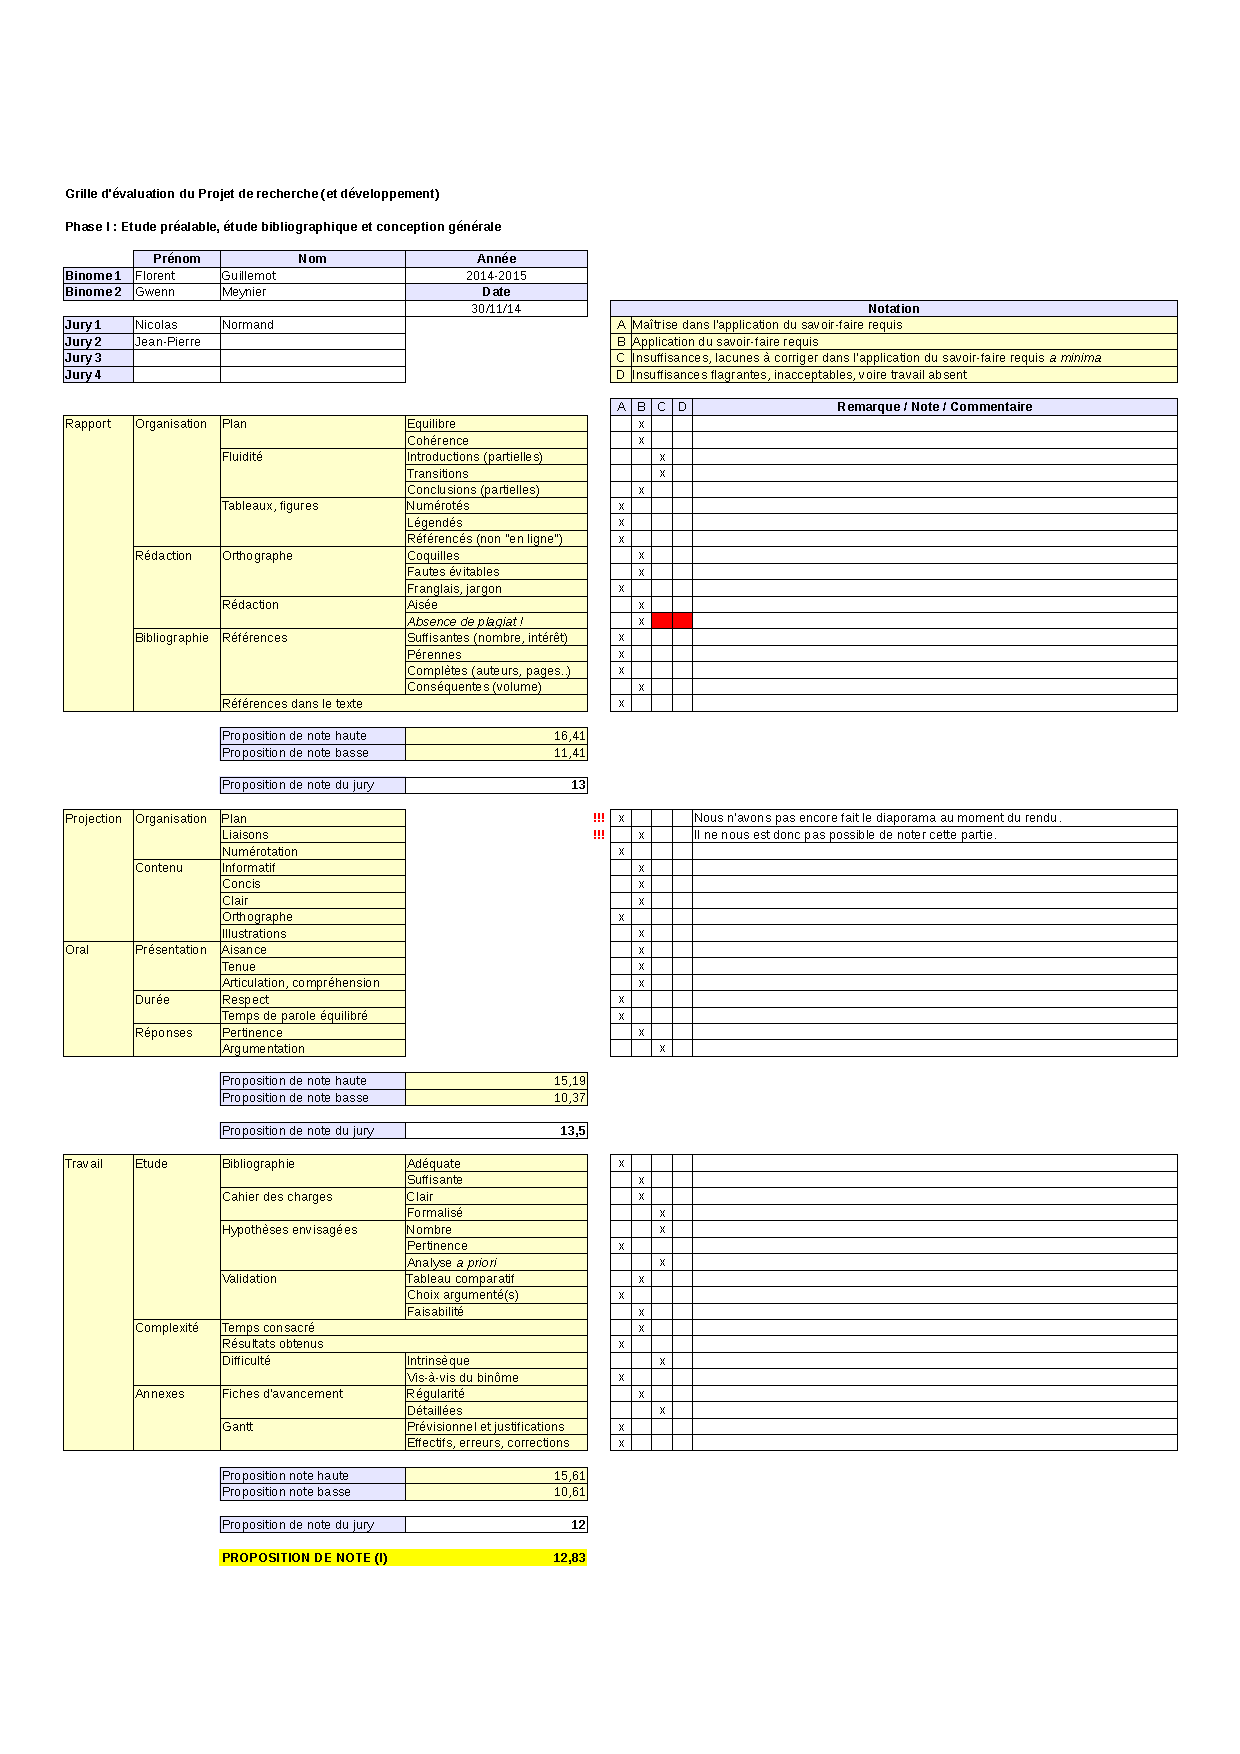
\includegraphics[width=0.9\textheight]{Images/Grille-Evaluation-PRD1}}
      \else
         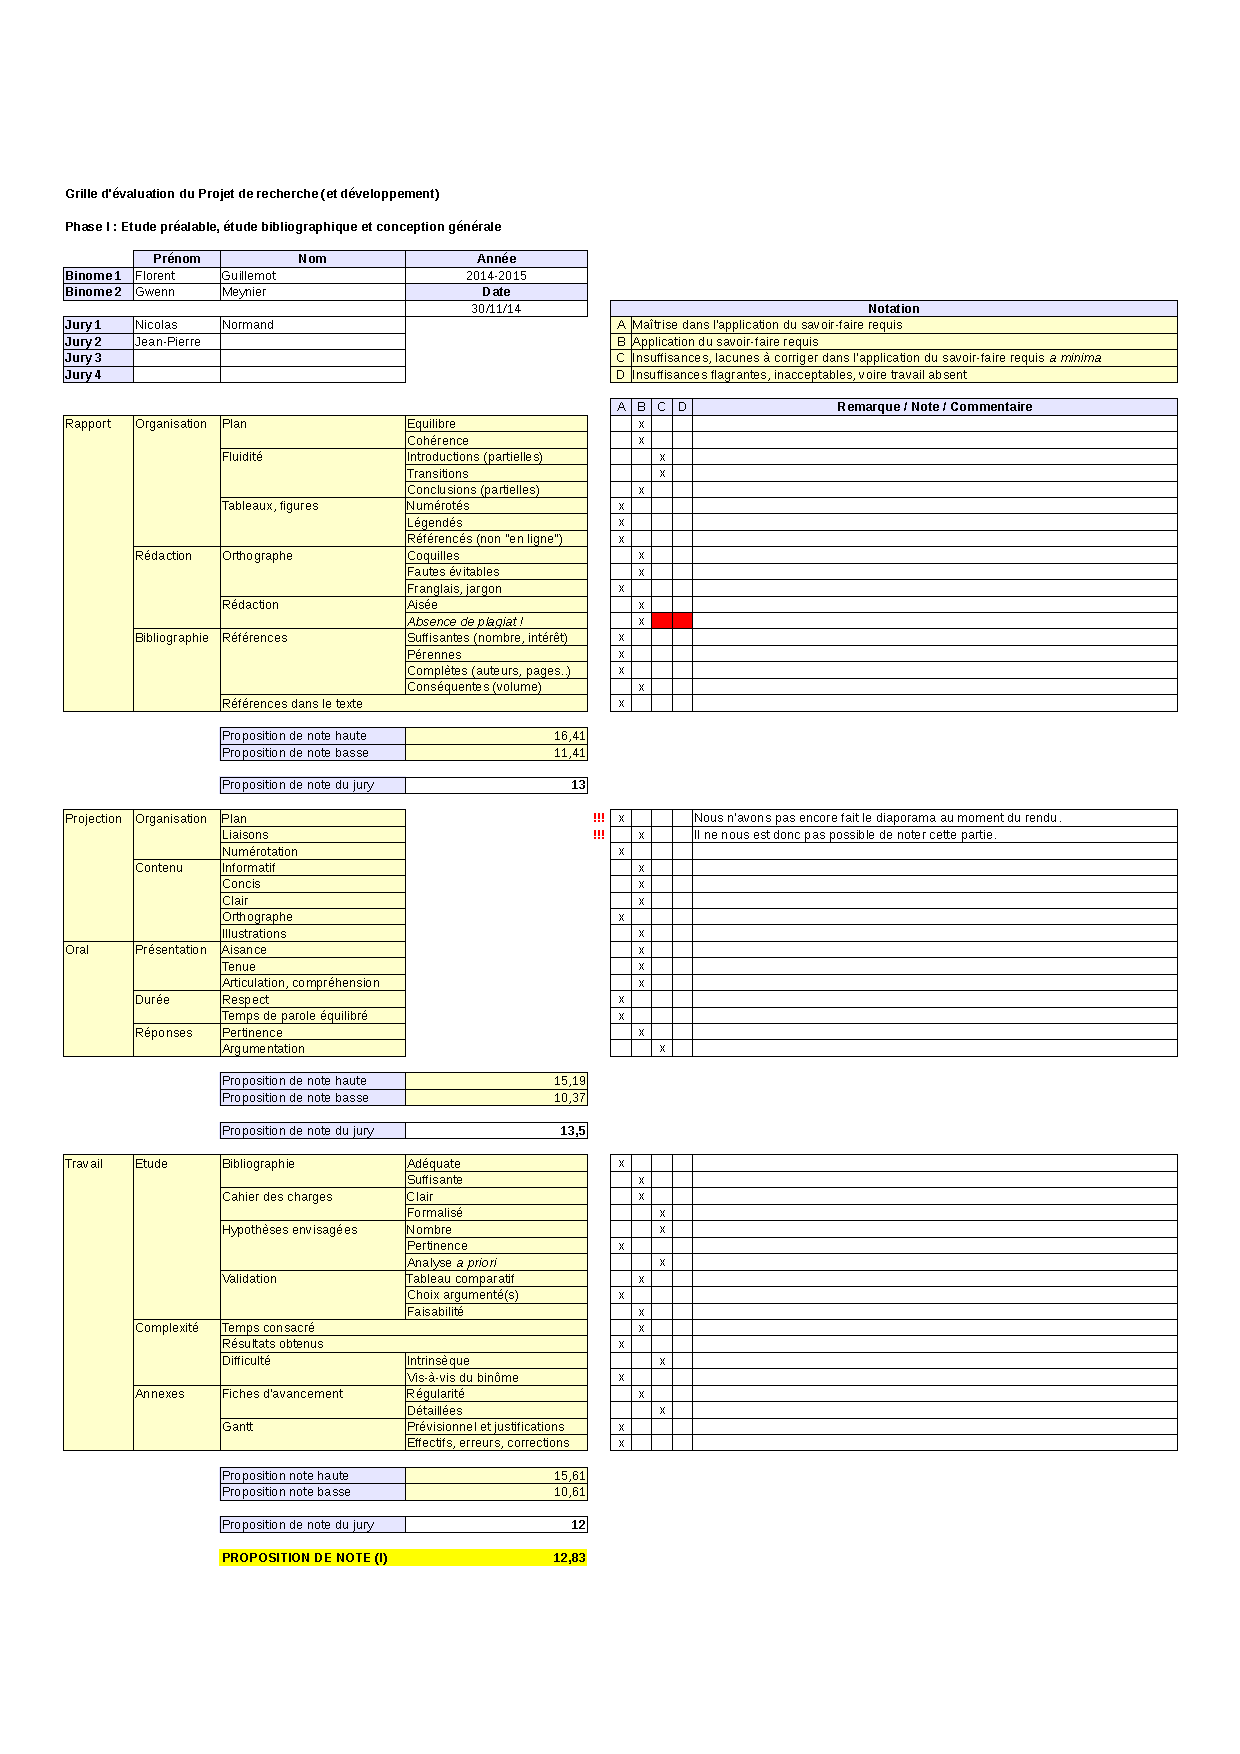
\includegraphics[width=0.9\textwidth]{Images/Grille-Evaluation-PRD1}
      \fi
	\caption{Points à contrôler à l'issue de la phase I}
	\label{fig:AutoEvaluationTravailIntermediaire}
\end{figure*}

La figure~\ref{fig:AutoEvaluationTravailFinal} permet d'énumérer un certain nombre de points importants dans les trois composantes du travail ainsi que d'évaluer notre niveau de satisfaction à l'issue de la phase~II, constituée de :
\begin{enumerate}
	\item la conception détaillée ;
	\item la réalisation ;
	\item la recette.
\end{enumerate}

\begin{figure*}
	\centering
      \ifscreen
         \rotatebox{90}{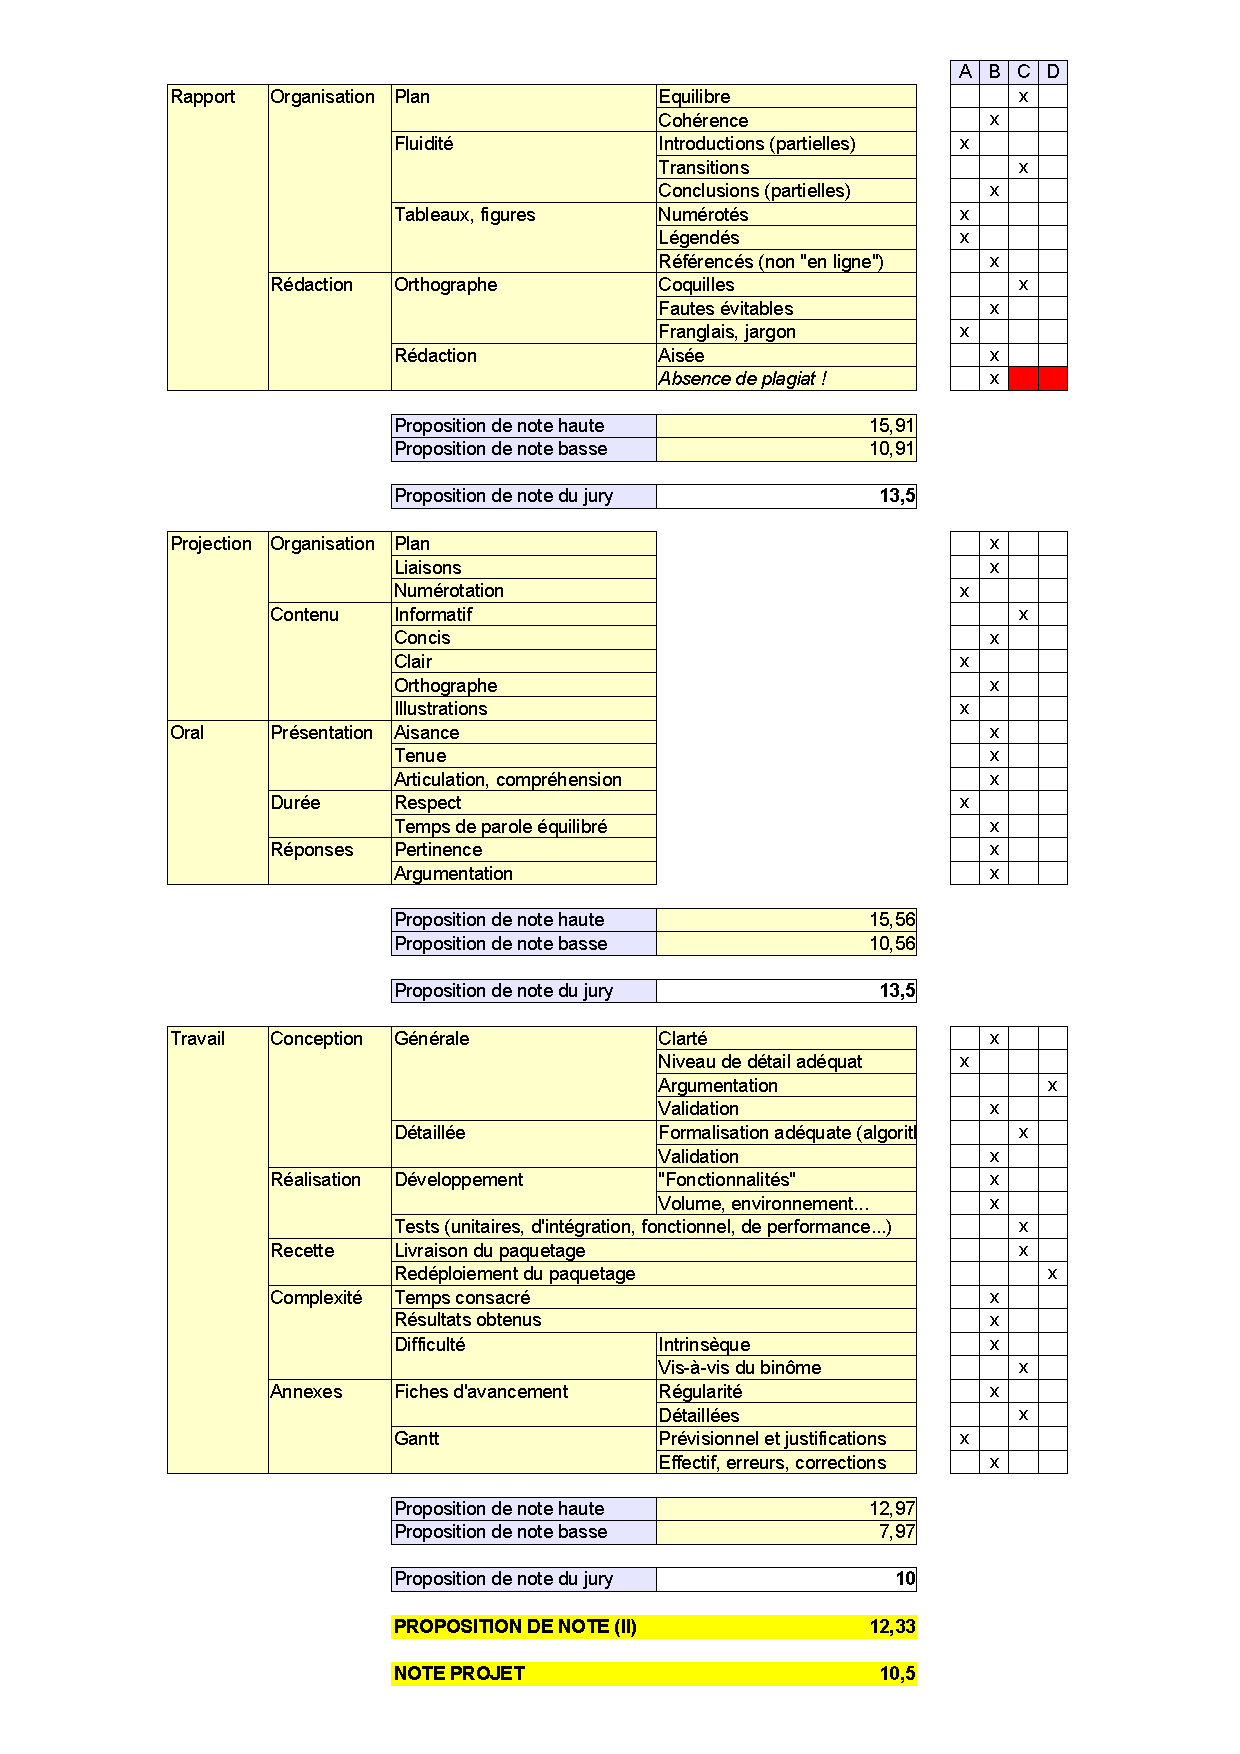
\includegraphics[width=0.9\textheight]{Images/Grille-Evaluation-PRD2}}
      \else
         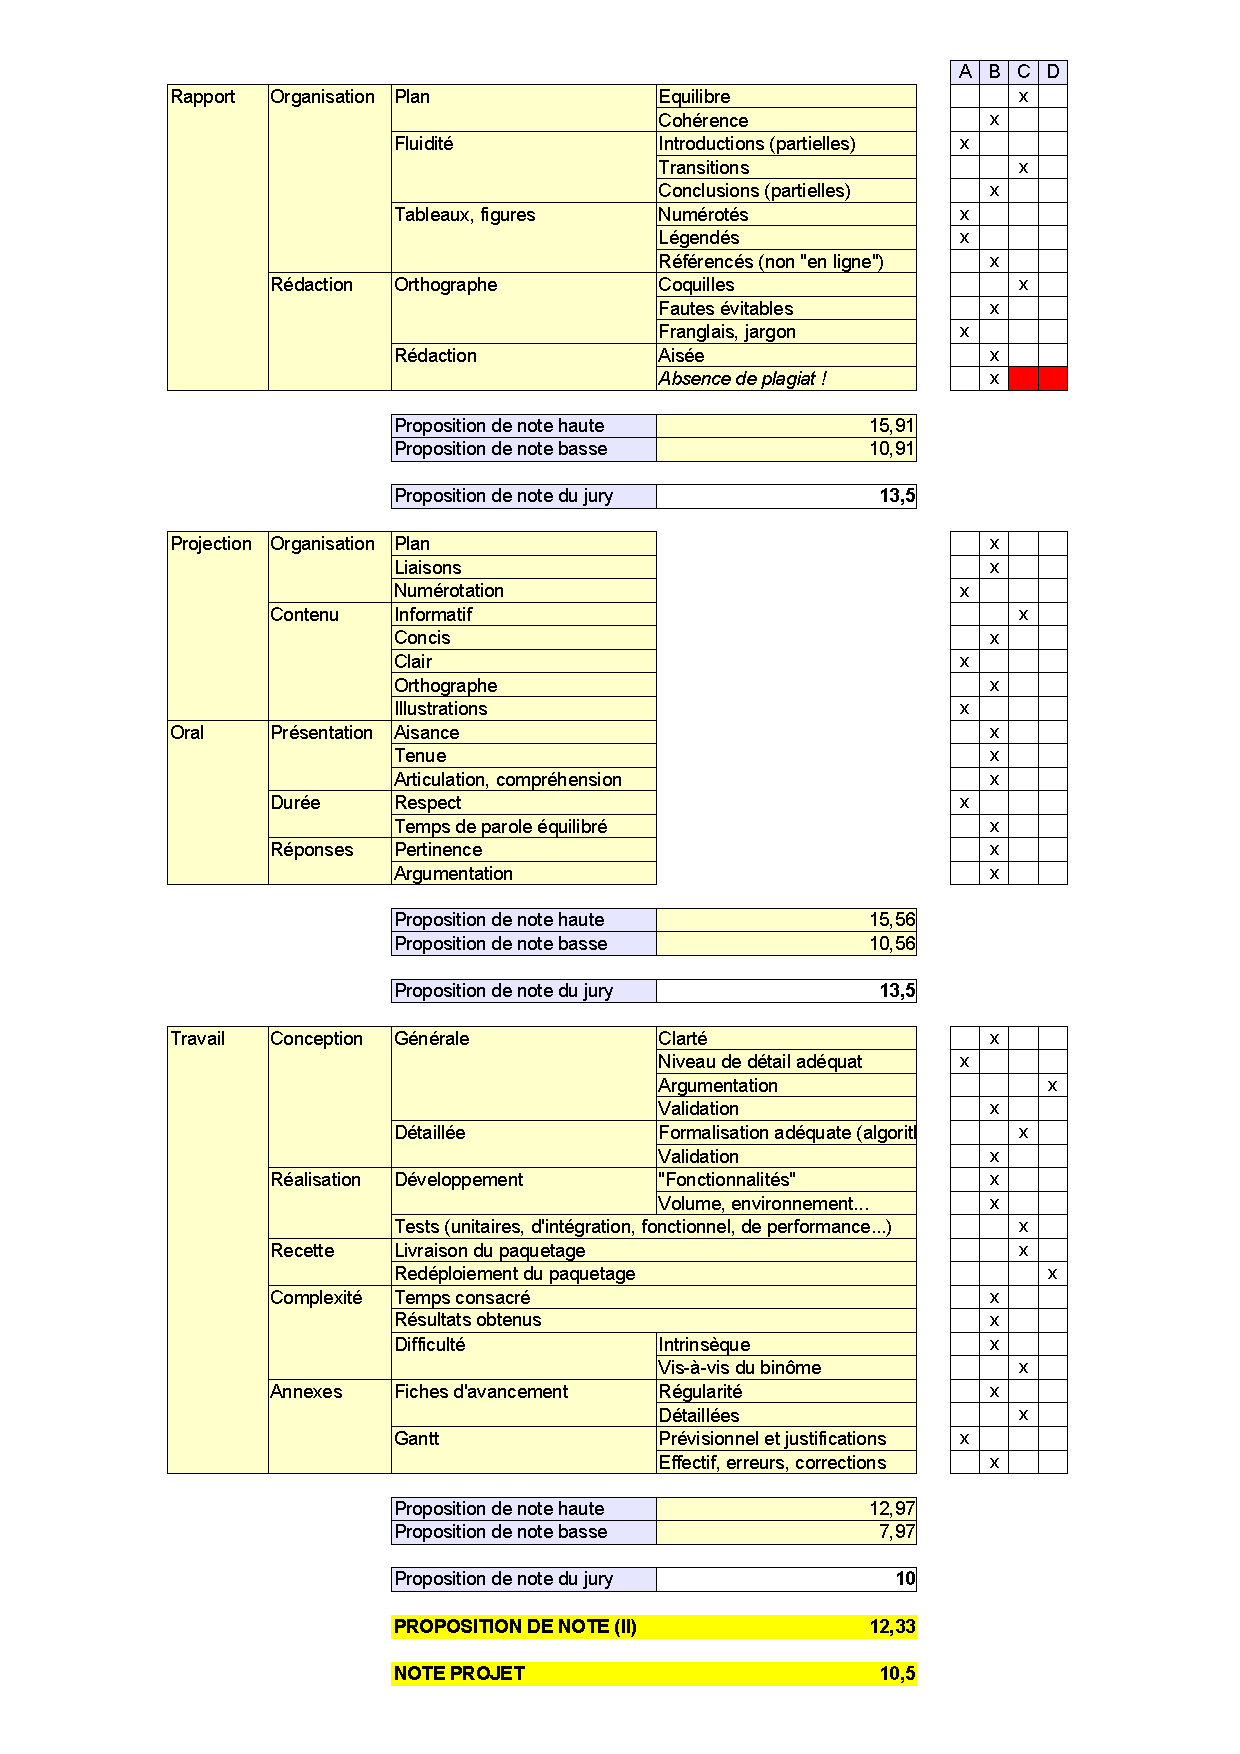
\includegraphics[width=0.9\textwidth]{Images/Grille-Evaluation-PRD2}
      \fi
	\caption{Points à contrôler à l'issue de la phase II}
	\label{fig:AutoEvaluationTravailFinal}
\end{figure*}

\end{document}
